\section{Component Type Hierarchy}
\label{sec:ComponentTypes}

Introduce types for substitutability of components

Most of today's component meta models do not clearly distinguish between a
component and its type. Often, the difference between both concepts is
not clarified. Furthermore, the conformance of a component to a type is not
defined. So the introduced concepts are very vague and only a few knowledge
about the substitutability of a component exists.

\begin{quote}
``As such, a component serves as a type whose conformance is defined by these
provided and required interfaces $[\ldots]$. One component may therefore be
substituted by another only if the two are type conformant
\cite[p.142]{OMGUML2005a}.''
\end{quote}

Here, the terms \emph{component type} and \emph{conformance} of components and
types are mentioned. However, both concepts are not further clarified. 

There are mainly two different concepts of component types. Both differ in
their interpretation of substitutability. 

The first one originates from object
oriented software development. There, a class can be substituted by another if
it implements at least the same interfaces. Translating this view to the
world of software components, a component can be substituted by another if it
offers at least the same set of provided interfaces.

The second one does not only consider provided interfaces, but also the
required interfaces of a component.

Depending on the task, both concepts have their advantages and disadvantages.
Thus, we do not want to limit on one of the concepts.

Both schools specify the required interfaces of a software component. However,
the interpretation of a required interface is completely different.

So far, we identified three different meanings of the specified required
interfaces of a type:
\begin{enumerate}
\item	A required interface can be used, but additional interfaces can be
added.
\item	Only the listed required interfaces can be used.
\item	A required interface has to be used in a predefined way and certain call
sequences have to be executed. 
\end{enumerate}

Required interfaces of the provided-type are not considered explicitly. However,
if they are specified, their meaning corresponds to the first case in the list,
since, for provided-types, the use of external services is not limited. The
second case corresponds to the complete-type. The usage of external services is
limited to the required interfaces specified for the component and no further
interfaces can be used by the component. The last case expresses additional
component requirements. For example, we could specify that all information has
to be stored in a database. So, the interface of the database must be called
using certain call sequences.

The Palladio Component Meta Model combines the two schools for component types
and the different meanings of required interfaces to provide a more flexible
type system for components.

\begin{figure}[htbp]
\centering
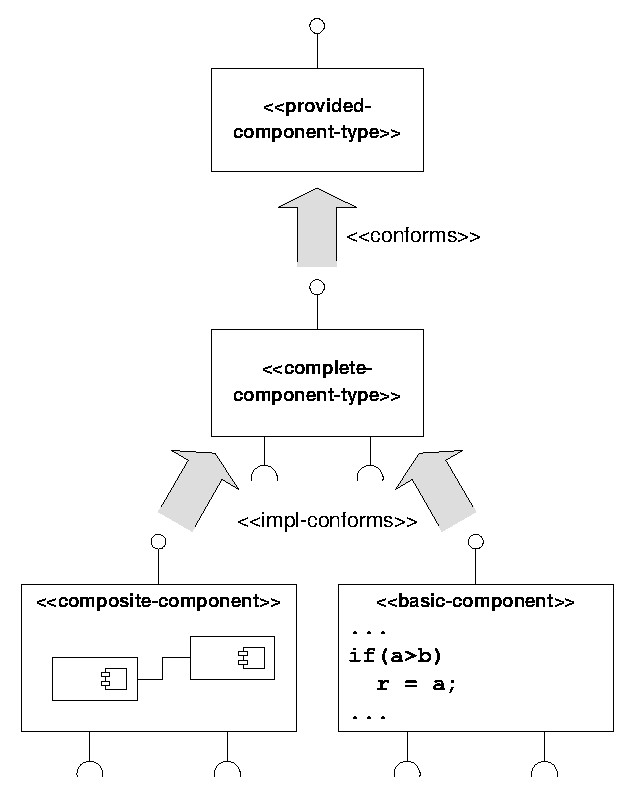
\includegraphics[width=3.3in]{example/Overview_TypeHierarchie}
\caption{Different type levels of a software component.}
\label{fig:TypeOverview}
\end{figure}

Figure \ref{fig:Tig:TypeOverview} shows the component type
hierarchie of the Palladio component meta modell.
<<provided component-type>>
<<complete component-type>>
component implementation description
<<basic component>> <<composite component>>


\subsection{Web Server}
In the following, we describe the concepts mentioned above in more detail. To do
so, we use the architecture of a prototypical web server shown in figure
\ref{fig:WebserverComponents}. The web server has been implemented in C\# for
the .Net 1.1 framework. It consists of a set of components that
communicate via a clear defined set of interfaces only. -- Architecture good
for reasoning about software components.

\begin{figure}[htbp]
\centering
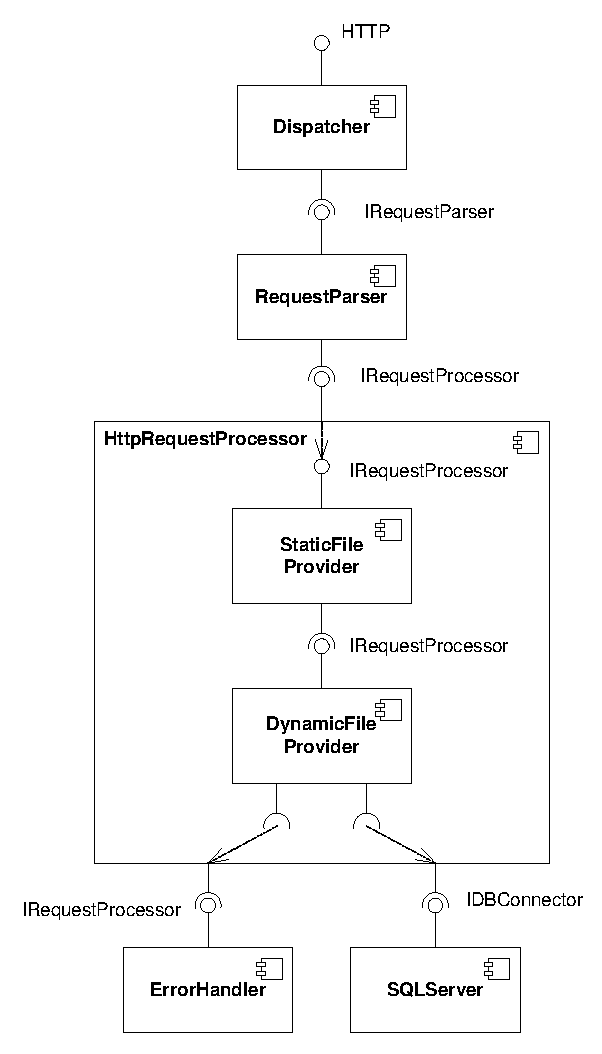
\includegraphics[width=3.3in]{example/WebserverComponents}
\caption{Component architecture of a web server.}
\label{fig:WebserverComponents}
\end{figure}

The main part of the web server is realised by three components: Dispatcher,
RequestParser, and HttpRequestProcessor. The Dispatcher listens for connections.
For each incoming HTTP request, it spawns a new tread and
activates the RequestParser. The parser analyses the request and passes the
result to the HttpRequestProcessor. The request processor is organised as a
chain of responsability \cite{gamma1995a}. Each of its subcomponents checks
whether it can handle the incoming request. If so, it returns the result,
otherwise it passes the request to the next component in the chain of
responsibility. The ErrorHandler represents the end of the chain and returns an
error message if the request could not be handled by any of the components.
Additionally, the SQLServer is required to create dynamic HTML pages.

\subsection{Component Implementation Description}
This is what most software engineers think of if they are talking about
software components.

A component implementation description is always associated with a real
component implementation binary component. Certainly, multiple implementations
can exist for a single description, implementing the component in different
languages like Java and C\# and technoligies, like Corba, J2EE, or .Net.

different specifications

UML the implementation of a component is described by a set of classes and
their interactions. 

Parametric contracts need a different view. They specifiy the dependency of
provided an required interfaces by means of service effect specifications.

Since our main aim is the prediction of QoS, we focus on the description using
parametric contracts in this articel. However, any kind of implementation
description is possible.

Different implementation desriptions are possible.
Composite components
Basic components

In general, a component model does not provide any information about the inner
structure of its components, since components are regarded as a black-box
entities. However, black-box components inhibit the analysis of Quality of
Service (QoS) attributes of the system, since important information about the
dependency of these attributes on external services, hardware and software
resources, and the usage profile cannot be specified.  With black-box
components, only static QoS contracts, like the ones specified by the QoS
Modelling Language (QML) \cite{frolund1998a}, can be used, but these are not
sufficient for this task. If the required QoS profile of a component cannot be
provided by its environment, the component is likely to work, but with lower
quality. Therefore, we need additional information on the inner
structure to analyse QoS attributes of a component in dependence on its
environment at design time.

A \emph{basic component} represents a basic block that is not further
subdivided. It implements a certain functionality and is defined by its provided
interfaces, required interfaces, and service effect specifications.


The fact that a basic component represents a single block does not imply that
the real implementation hast to be one 'block' as well. Since we are talking
about the implementation description and not the actual implementation, this
difference is possible and actually desired in some cases. For example, the
actual implementation of a component might consist of a set of classes and/or
subcomponents. This information is abstracted away in the description as a basic
component. So, the description of a basic component only represents one view on
a software component. Another view on a component are, for example, a class
diagram or its source code.

A \emph{composite component} consists of a set of interconnected subcomponents
that realise its functionality. 

The HttpRequestProcessor of the web server architecture.

As described in section \ref{sec:ComponentTypes}, a component implementation
conforms to a complete-type if it offers at least the functionality specified
in by the provided interfaces of the complete type and does not require more
functionality than specified in the required interfaces of the complete-type.

\subsection{Complete Component Type}

\begin{figure}[htbp]
\centering
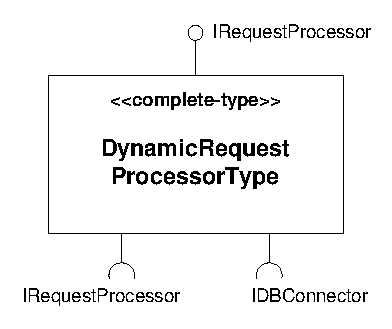
\includegraphics[scale=0.85]{example/DynamicRequestProcessorType}
\caption{Component type for dynamic request processors.}
\label{fig:DynamicRequestProcessorType}
\end{figure}

Looking at the architecture of the web server, we can identify different
complete component types. For example, the components HttpRequestProcessor and
DynamicFileProvide provide the IRequestProcessor interface and use the
interfaces IDBConnector and IRequestProcessor. The first one is used to create
dynamic content of web pages. The second one is required to forward the request
to the next component in the chain of responsibility. The corresponding type of
both components is shown in figure \ref{fig:DynamicRequestProcessorType}.

\begin{figure}[htbp]
\centering
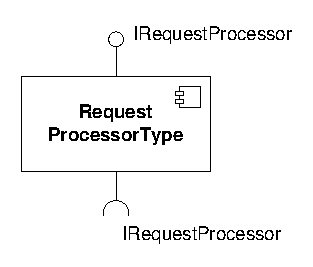
\includegraphics[scale=0.85]{example/RequestProcessorType}
\caption{Another component type used in the web server.}
\label{fig:RequestProcessorType}
\end{figure}

The type of the StaticFileProvider component shown in figure
\ref{fig:RequestProcessorType} provides and requires the IRequestProcessor
interface only. So, it differs from the DynamicRequestProcessorType, which
additionally requires the IDBConnector interface. 

The types shown in figures \ref{fig:DynamicRequestProcessorType} and
\ref{fig:RequestProcessorType} are derived from existing components and describe
their complete provided and required functionality.
It is obvious that a component conforms to a type if it provides and requires
exactly the interfaces specified by the type. However, this is not the case in
general. A component is likely to differ from its more general type, but,
nevertheless, still be conformant to the type. So, when does a component conform
to a type?

<<implementation-conforms>>
A component conforms to a type, if it offers at least the functionality
specified by the provided interfaces of the type and uses only the functionality
specified by the required interfaces of the type.

For example, a component must offer the IRequestProcessor interface to conform
to one of the types in figure \ref{fig:DynamicRequestProcessorType} or
\ref{fig:RequestProcessorType}, but it can provide additional interfaces.
Furthermore, a component can only use services that are specified in the
required interfaces of the type. The DynamicFileProvider does not conform to the
RequestProcessorType, since it uses the IDBConnector interface. Note that a
component does not have to use all required interfaces of its type. So, all
components that conform to the RequestProcessorType also conform to the
DynamicRequestProcessorType, since they do not require the
IDBConnectorInterface. 

The definition of conformance corresponds to the view on required and provided
interfaces as pre- and postconditions of components. The precondition can only
be weakened. Thus, the component implementation must not use interfaces other
than the required interfaces specified by the type. Furthermore, the
postcondition can only be strengthened. The component can offer any interfaces,
but it must at least provide the ones specified by the type. With this notion of
conformance, the type system of components is contravariant.

This understanding of conformance between components and types allows us to
define substitutability of components. A component \texttt{A} can be substituted
by a component \texttt{B} if \texttt{B} conforms to the type defined by
\texttt{A}. The type defined by a component includes all its provided and
required interfaces. This is a very pessimistic definition of substitutability,
which can be weakened under certain conditions. 

\subsection{Provided Component Type}

In many cases, we are not only interested in the substitution of complete
components including provided and required interfaces, but in a substitution
with respect to provided interfaces only. This is the case if the functionality
is more important than the requirements of a component or if we compare the
functionality offered by different components. Furthermore, it might not be
possible to specify all required interfaces of a component in advance. 

\begin{figure}[htbp]
\centering
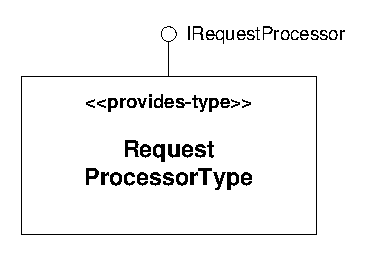
\includegraphics[scale=0.85]{example/ProvidesType}
\caption{provided-type of the RequestProcessorType and
DynamicRequestProcessorType.}
\label{fig:ProvidesType}
\end{figure}

Hence, we want to allow conformance with respect to provided interfaces only.
Therefore, we introduce a \emph{provided-type} which only considers provided
interfaces. The provided-type of the RequestProcessortType and the
DynamicRequestProcessorType is shown in figure \ref{fig:ProvidesType}. 
It represents a more abstract view on software components. This is needed,
since, during design time, it is often not clear what other components will be
needed to implement the desired functionality. Expecting the software architect
to decide this would require nearly the same effort as implementing the software
component. Thus, the development process of a component should not be fixed to
the required interfaces specified by a component type. It rather evolves with
the development of the component. Provided and required interfaces are added and
removed over time. The system architect specifies a basic set of interfaces that
is used by the components to communicate. More interfaces might be added later
to implement the functionality of the components.


The distinction of provided- and complete-types brings several advantages. By
provided-types, we gain a high flexibility during software development.
Furthermore, we can define a substitutability focussing on the functionality of
a component. On the other hand, complete-types define a strict substitutability.
If a component is replaced by another and both conform to the same complete
type, we can assure that certain classes of interoperability problem cannot
occur. Moreover, complete-types allow a complete specification of the externally
visible behaviour of a software component. The co-existence of both concept
offers a high flexibility in software architecture design.

\subsection{The Component Type Hierarchy}

\begin{figure}[htbp]
\centering
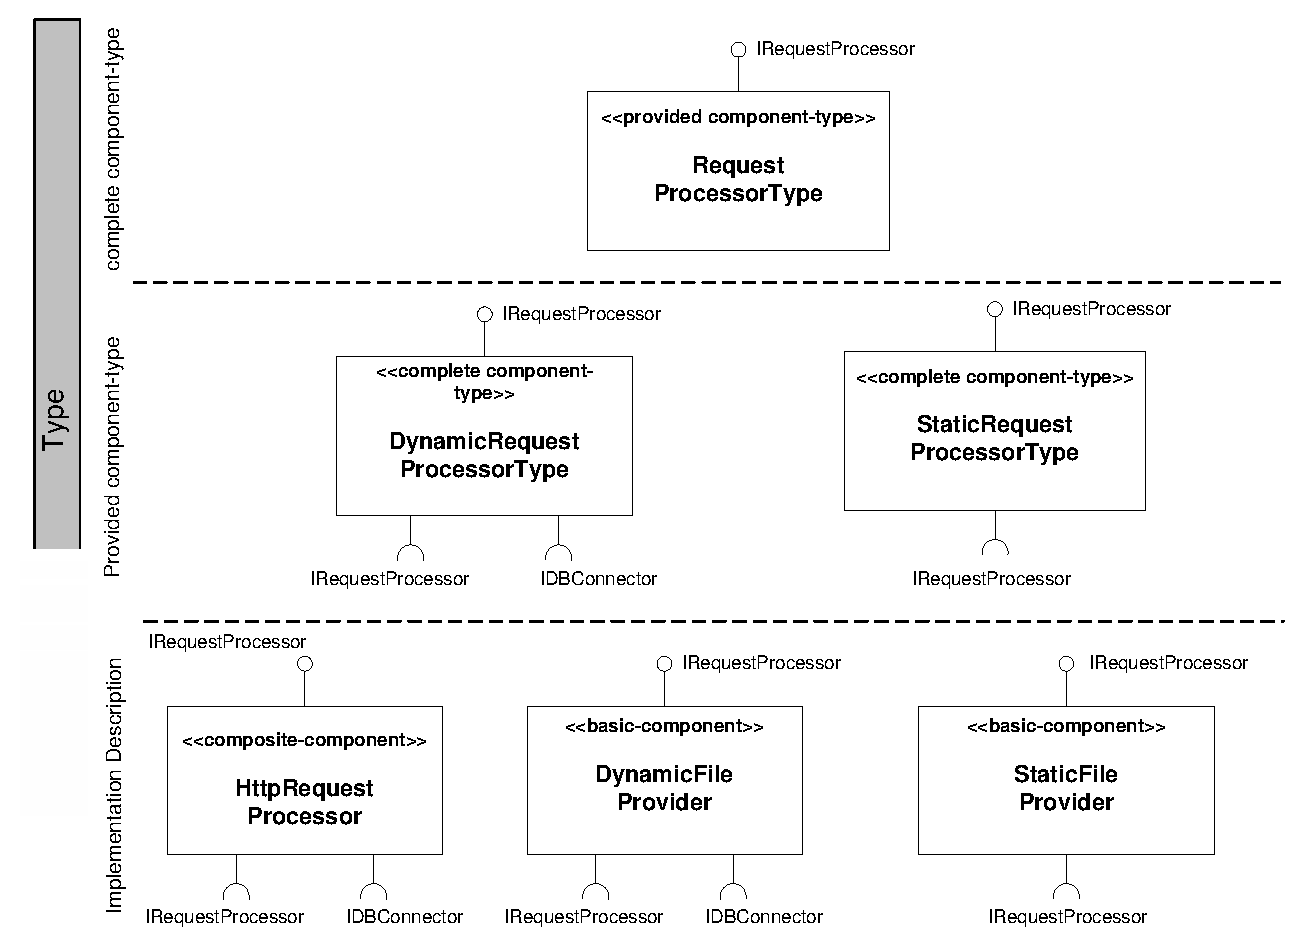
\includegraphics[width=3.3in]{example/TypeHierachy}
\caption{Type Hierarchie}
\label{fig:WebserverComponents}
\end{figure}

Figure \ref{fig:TypeHierarchy} gives an overview of the relation of
provided-types, complete-types and component implementation descriptions.
TODO:Figure and description

With the implementation description of software components, we have enough
information to compute QoS attributes of the component in dependence on external
services.
TODO:Example

